\chapter{Hình học giải tích}

\section{Theo dòng lịch sử}

Hình học xuất hiện từ thời xa xưa, xuất phát từ những nhu cầu thực tế nhất của con người là đo đạc để phân chia đất đai, xây dựng, canh tác, ... Từ đó con người đã có nhận thức rất sớm về quan hệ song song và vuông góc giữa hai đường thẳng.

Một cách hình ảnh (mà thật ra hình học là môn học về hình ảnh) thì hai đường thẳng song song không cắt nhau dù có kéo dài chúng ra vô tận. Các đường thẳng song song luôn có nhiều điều thú vị, cả ở mặt phẳng Euclid lẫn trong không gian. Đầu tiên phải kể đến định lý mang tên triết gia vĩ đại của Hy Lạp: Thales.

\subsection*{Thales của Miletus}

Thales của Miletus được cho rằng sinh vào khoảng năm 624 Trước Công nguyên (TCN) và mất năm 547 TCN tại Miletus (Thổ Nhĩ Kì ngày nay)\footnote{https://mathshistory.st-andrews.ac.uk/Biographies/Thales/}.

\begin{figure}[ht]
	\centering
	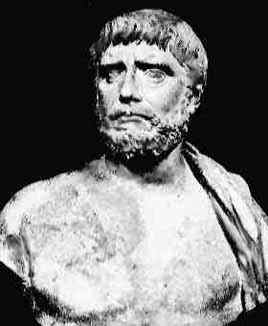
\includegraphics[scale=0.5]{analytic_geometry/Thales.jpeg}
	\caption{Thales của Miletus}
\end{figure}

Ông được xem là nhà triết học đầu tiên khi không cố gắng giải thích tự nhiên bằng thần thoại hay các thế lực siêu nhiên như trước. Trường phái triết học do ông sáng lập, trường phái Milet, cho rằng mọi vật có nguồn gốc từ nước. Nhà triết học nổi tiếng Aristotle đánh giá rằng Thales là người sáng lập ra \textit{triết học duy vật sơ khai}.

Trong toán học, Thales được biết tới với định lý mang tên ông về các đường song song. Định lý Thales được phát biểu như sau:

\begin{theorem}[Định lý Thales]
    Trong một tam giác, đường thẳng song song với một cạnh chắn trên hai cạnh còn lại các đoạn thẳng tương ứng tỉ lệ.
\end{theorem}

\begin{figure}[ht]
	\centering
	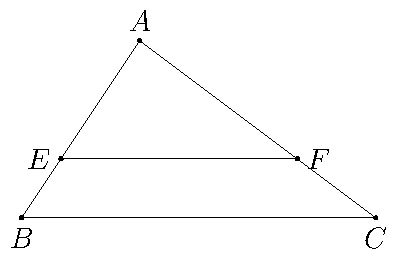
\includegraphics{analytic_geometry/thales1.pdf}
	\caption{Định lý Thales trên mặt phẳng}
	\label{thales1}
\end{figure}

Theo định lý Thales, nếu $EF$ song song với $BC$ thì ta có $\dfrac{AE}{AB} = \dfrac{AF}{AC} = \dfrac{EF}{BC}$ (hình \ref{thales1}).

Không dừng lại ở mặt phẳng, khi mở rộng lên không gian định lý Thales cũng cho chúng ta một kết quả quan trọng khi nói tới các mặt phẳng song song nhau.

\begin{theorem}[Định lý Thales trong không gian]
    Trong khối chóp, mặt phẳng song song mặt đáy chắn các cạnh nối từ đỉnh hình chóp tới các đỉnh của mặt phẳng đáy các đoạn thẳng tương ứng tỉ lệ.
\end{theorem}

\begin{figure}[ht]
	\centering
	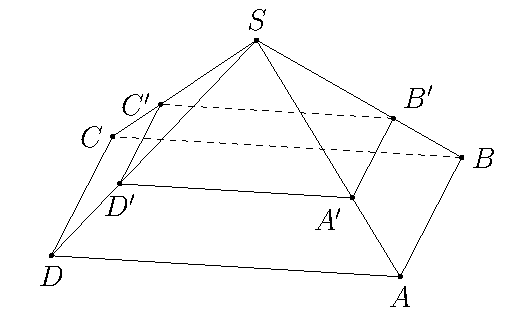
\includegraphics{analytic_geometry/thales2.pdf}
	\caption{Định lý Thales trong không gian}
	\label{thales2}
\end{figure}

Theo định lý Thales, nếu mặt phẳng $(ABCD)$ song song với mặt phẳng $(A'B'C'D')$ thì $\dfrac{SA}{SA'} = \dfrac{SB}{SB'} = \dfrac{SC}{SC'} = \dfrac{SD}{SD'}$ (hình \ref{thales2}).

\subsection*{Pythagoras của Samos}

Khi nhắc tới vuông góc, chúng ta thường nhớ tới định lý ngày nào được học ở thời học sinh: định lý Pythagoras. Định lý này nói về quan hệ giữa độ dài các cạnh trong một tam giác vuông. Định lý tuy đơn giản nhưng có ý nghĩa rất quan trọng trong đời sống và khoa học của con người suốt chiều dài lịch sử. Đây cũng là tiền đề cho định lý mang tính lịch sử của nhân loại: định lý cuối cùng của Fermat.

\begin{figure}[ht]
	\centering
	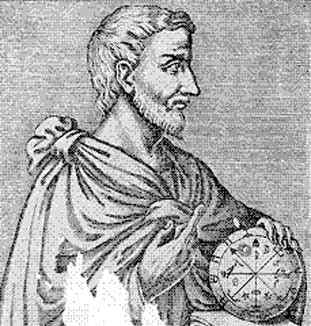
\includegraphics[scale=0.5]{analytic_geometry/Pythagoras.jpeg}
	\caption{Pythagoras của Samos}
\end{figure}

Pythagoras của Samos cũng là nhà triết học Hy Lạp cổ, được cho rằng sinh vào khoảng năm 570 TCN và mất năm  490 TCN\footnote{https://mathshistory.st-andrews.ac.uk/Biographies/Pythagoras/}. Ông được học tập từ nhà triết học Thales và cũng có nhiều đóng góp cho sự phát triển của toán học, thiên văn học và âm nhạc. Tuy nhiên khác với thầy mình, trường phái triết học của ông cho rằng những con số là nguồn gốc của vạn vật và sử dụng những con số để giải thích những hiện tượng khoa học. Từ đây, các lý thuyết về âm nhạc được ra đời, cụ thể là các mối liên hệ về tần số với sự rung của dây nhạc cụ.

Ông là một trong những người hiếm hoi cho phép cả phụ nữ đi học ở lớp của mình vào thời ấy. Điều đó giúp phổ biến toán học nói riêng và kiến thức nói chung tới nhiều tầng lớp nhân dân. Tuy nhiên ông cũng có một hội kín rất thú vị. Như đã nói ở trên, trường phái triết học Pythagoras cố gắng giải thích nguồn gốc vạn vật bằng những con số. Điều này đã dẫn họ tới những khám phá động trời vào thời ấy.

Một trong những khám phá đó là về sự tồn tại của số vô tỉ dựa vào định lý mang tên ông. Lịch sử đã chỉ ra rằng trước Pythagoras, người Babylon và Ai Cập đã tìm ra rất nhiều bộ số nguyên $(a, b, c)$ thỏa mãn $a^2 + b^2 = c^2$ là độ dài ba cạnh tam giác vuông. Định lý Pythagoras mà ngày nay chúng ta biết được phát biểu rằng:

\begin{theorem}[Định lý Pythagoras]
    Trong một tam giác vuông, bình phương độ dài cạnh huyền bằng tổng bình phương độ dài hai cạnh góc vuông.
\end{theorem}

Như vậy nếu gọi độ dài cạnh huyền là $c$, độ dài hai cạnh góc vuông lần lượt là $a$ và $b$ thì $a^2 + b^2 = c^2$ (hình \ref{pythagoras1}).

\begin{figure}[ht]
	\centering
	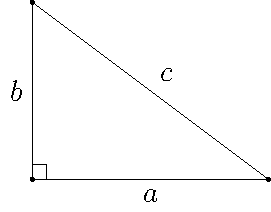
\includegraphics{analytic_geometry/pythagoras1.pdf}
	\caption{Định lý Pythagoras}
	\label{pythagoras1}
\end{figure}

Nếu $a = b = 1$ thì sao? Khi đó bình phương độ dài cạnh huyền $c^2 = 2$. Tuy nhiên không thể tìm ra một số hữu tỉ nào để bình phương lên là 2 cả. Phát hiện này là một chấn động đối với thời Pythagoras và ông yêu cầu tất cả thành viên trong hội phải giữ kín bí mật về sự phát hiện này. Tuy nhiên thông tin vẫn lọt ra ngoài và truyền thuyết kể rằng ông đã xử tội chết cho thành viên của hội không tuân thủ.

Pythagoras đã đưa một khái niệm cực kì quan trọng trong toán học, gọi là \textit{chứng minh} (proof). Để chứng minh một mệnh đề là đúng, chúng ta cần các mệnh đề (thường đơn giản hơn) đúng trước đó. Bằng các phép suy luận thích hợp dựa trên các mệnh đề đúng trước đó, chúng ta có thể kết luận rằng mệnh đề cần chứng minh là đúng. Phép chứng minh có thể gọi là \textit{xương sống} của toán học, vì nếu không có một phép chứng minh đúng đắn thì một mệnh đề không thể được xác định được là có đúng hay không. Trong trường hợp của Fermat, khi ông đưa ra định lý Fermat nhưng không kèm chứng minh (vì lề sách quá chật nên không viết lời giải được) thì chúng ta không thể biết định lý Fermat có đúng hay không (?).

Nếu việc suy luận dựa trên các mệnh đề, hoặc định lý, đã đúng trước đó, thì phải có một lúc nào đó việc này dừng lại. Chúng ta không thể suy ngược tới vô hạn lần được. Do đó chúng ta cần những mệnh đề luôn đúng nhưng tính đúng đắn của nó được kiểm nghiệm trong thực tiễn. Chúng được gọi là \textit{tiên đề} (axiom). Nhân vật tiếp theo được đề cập tới sẽ dẫn chúng ta tới hệ thống tiên đề làm nền tảng cho hình học.

\subsection*{Euclid của Alexandria}

Đúng vậy, Euclid là người đặt nền móng cho hình học với bộ sách nổi tiếng \textit{Elements} của mình. Trong bộ sách này đề cập tới những tiên đề, định lý làm nền tảng cho bộ môn hình học và vẫn còn ý nghĩa cho tới tận ngày nay. Những gì viết trong đó không quá xa lạ với những gì được giảng dạy trong nhà trường.

\begin{figure}[ht]
	\centering
	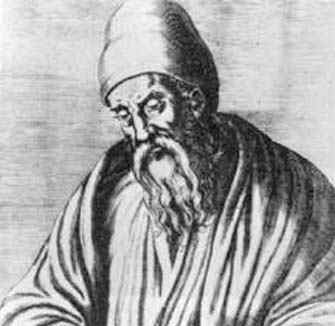
\includegraphics[scale=0.5]{analytic_geometry/Euclid.jpeg}
	\caption{Euclid của Alexandria}
\end{figure}

Euclid của Alexandria sinh vào khoảng năm 325 TCN và mất vào khoảng năm 265 TCN\footnote{https://mathshistory.st-andrews.ac.uk/Biographies/Euclid/}. Thông tin về ông không có nhiều. Nhưng chỉ mỗi bộ sách \textit{Elements} cũng đủ để người đời sau cho rằng ông là người có ảnh hưởng nhất trong 2000 năm lịch sử phát triển của toán học.

Năm tiên đề cơ bản của hình học được ông phát biểu trong bộ \textit{Elements} được phát biểu như sau:

\begin{enumerate}
	\item Qua hai điểm bất kì luôn vẽ được một đường thẳng
	\item Đường thẳng có thể kéo dài vô hạn về cả hai phía
	\item Ta có thể xác định một đường tròn bằng tâm và bán kính của nó
	\item Mọi góc vuông đều bằng nhau
	\item Nếu một đường thẳng cắt hai đường thẳng khiến tổng hai góc trong cùng phía nhỏ hơn hai vuông thì hai đường thẳng đó chắc chắn sẽ cắt nhau tại một điểm nào đó
\end{enumerate}

Tiên đề số 5 là rắc rối và phức tạp nhất. Nó không thực sự tự nhiên và có nhiều sự vướng mắc. Đây chính là tiên đề cho sự ra đời của hình học phi-Euclid hơn 1500 năm sau.

Bộ \textit{Elements} của Euclid bao gồm 13 quyển. Trong đó đề cập tới rất nhiều vấn đề của hình học, từ những phần tử đơn giản nhất cấu tạo nên hình học là điểm, đoạn thẳng, đường thẳng, tới những hình học lớn hơn như hình chữ nhật, hình tròn, đa giác, mặt phẳng. Thậm chí ông cũng đã có những dấu chân ở hình học không gian như hình chóp, hình cầu, hình nón (\cite{Euclid}, \cite{Casey2007}).

\section{Phương pháp tọa độ trong mặt phẳng}

Cuộc cách mạng trong hình học xảy ra khi nhà toán học lãng tử René Descartes phát minh ra hệ tọa độ và từ đó mọi đối tượng hình học có thể được biểu diễn bởi các phương pháp đại số như phương trình, đẳng thức.

\subsection*{Danh mục thuật ngữ và ký hiệu}

Đầu tiên chúng ta thống nhất các thuật ngữ cũng như ký hiệu được sử dụng kể từ đây.

\textbf{Điểm} là đơn vị cơ bản của hình học. Bất kì đối tượng hình học nào cũng là một \textit{tập hợp điểm}. Điểm được ký hiệu bởi chữ in hoa, ví dụ như $A$, $B_1$, $B_2$.

\textbf{Đường thẳng} đi qua hai điểm phân biệt cho trước. Đường thẳng có thể kéo dài vô hạn về hai phía. Đường thẳng được ký hiệu bởi chữ in thường hoặc chữ Hy Lạp trong ngoặc đơn, ví dụ như $(d)$, $(\Delta)$.

\textbf{Đoạn thẳng} chỉ phần đường thẳng nằm giữa hai điểm.

\textbf{Nửa đường thẳng} chỉ phần đường thẳng nằm một phía của một điểm trên đường thẳng và chỉ kéo dài vô hạn về phía đó.

\textbf{Vector} là đoạn thẳng có hướng. Với điểm đầu là $A$ và điểm cuối là $B$ thì vector từ $A$ tới $B$ được ký hiệu là $\overrightarrow{AB}$. Để chỉ một vector không cần biết điểm đầu và điểm cuối ta dùng chữ thường in đậm, ví dụ như $\bm{a}$.

\textbf{Góc giữa hai vector} $\overrightarrow{OA}$ và $\overrightarrow{OB}$ là góc $\angle AOB$ và ký hiệu là $(\overrightarrow{OA}, \overrightarrow{OB})$.

Tương tự đối với vector $\bm{a}$ và $\bm{b}$ thì góc giữa chúng ký hiệu là $(\bm{a}, \bm{b})$.

\subsection*{Vector trong mặt phẳng}

Trong hệ tọa độ $Oxy$ với tâm $O$ và hai trục $Ox$ (trục hoành) và $Oy$ (trục tung) vuông góc nhau, đặt $O = (0, 0)$ là tọa độ của tâm $O$.

Tiếp theo, mọi điểm trong mặt phẳng Euclid đi liền với cặp số $(x, y)$ chỉ tọa độ của điểm đó. Ví dụ $A = (1, 3)$, $B = (4, 1)$.

\begin{figure}[ht]
	\centering
	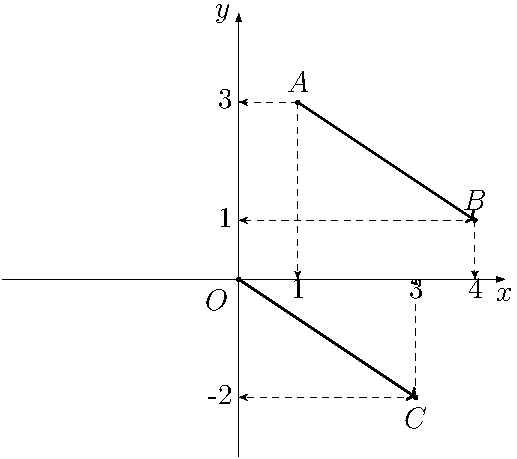
\includegraphics[page=1]{analytic_geometry/oxy1.pdf}
	\caption{Tọa độ của điểm trong mặt phẳng}
	\label{oxy1}
\end{figure}

Tọa độ của điểm cũng là tọa độ của vector từ $O$ tới điểm đó. Với hình \ref{oxy1} thì $\overrightarrow{OA} = (1, 3)$ và $\overrightarrow{OB} = (4, 1)$. Tọa độ của vector $\overrightarrow{AB}$ khi đó sẽ là $\overrightarrow{AB} = \overrightarrow{OB} - \overrightarrow{OA} = (4, 1) - (1, 3) = (3, -2)$. Cũng theo hình \ref{oxy1} thì ta thấy $\overrightarrow{AB} = \overrightarrow{OC} = (3, -2)$. 

Như vậy, nếu ta có hai điểm $A = (x_A, y_A)$ và $B = (x_B, y_B)$ thì vector $\overrightarrow{AB}$ là
\begin{equation}
	\overrightarrow{AB} = (x_B - x_A, y_B - y_A)
\end{equation}

\textbf{Tích vô hướng của hai vector} $\bm{a} = (x_1, y_1)$ và $\bm{b} = (x_2, y_2)$ được định nghĩa là
\begin{equation}
	\langle \bm{a}, \bm{b} \rangle = x_1 x_2 + y_1 y_2
\end{equation}

Ta cũng có thể ký hiệu tích vô hướng là $\bm{a} \cdot \bm{b}$.

Ta ký hiệu $\lVert \bm{a} \rVert$ là độ dài (chuẩn Euclid, Euclid norm) của vector $\bm{a}$. Trong hệ tọa độ Descartes vuông góc, theo định lý Pythagoras, độ dài của vector là độ dài cạnh huyền tam giác vuông (hình \ref{oxy1}). Như vậy, độ dài đoạn thẳng $AB$ với $A = (x_A, y_A)$ và $B = (x_B, y_B)$ là
\begin{equation}
	AB = \lVert \overrightarrow{AB} \rVert = \sqrt{(x_B - x_A)^2 + (y_B - y_A)^2}
\end{equation}

Khi đó cosin góc giữa hai vector $\bm{a}$ và $\bm{b}$ là
\begin{equation}
	\cos (\bm{a}, \bm{b}) = \frac{\bm{a} \cdot \bm{b}}{\lVert \bm{a} \rVert \cdot \lVert \bm{b} \rVert} = \frac{x_1 x_2 + y_1 y_2}{\sqrt{x_1^2 + y_1^2} \cdot \sqrt{x_2^2 + y_2^2}}
\end{equation}

Nếu góc giữa hai vector bằng 90 độ thì hai vector được gọi là vuông góc nhau. Khi đó tích vô hướng $\bm{a} \cdot \bm{b} = 0$.

\subsection*{Phương trình đường thẳng trong mặt phẳng}

Theo tiên đề Euclid, một đường thẳng được xác định khi biết hai điểm phân biệt thuộc đường thẳng đó. Trong hệ tọa độ, chúng ta có hai cách tìm phương trình đường thẳng.

\textbf{Bằng vector pháp tuyến}. Vector pháp tuyến của đường thẳng là vector vuông góc với mọi vector có phương là đường thẳng đó. Giả sử $\bm{v} = (a, b)$ là vector pháp tuyến của đường thẳng đi qua điểm $M_0 = (x_0, y_0)$. Khi đó đường thẳng đi qua qua $M_0$ nhận $\bm{v}$ làm vector pháp tuyến là \textit{tập hợp điểm} $M = (x, y)$ trên mặt phẳng sao cho $\bm{v} \cdot \overrightarrow{M_0 M} = 0$. Điều này tương đương với
\begin{equation}
	\bm{v} \cdot \overrightarrow{M_0 M} = a \cdot (x - x_0) + b \cdot (y - y_0) = 0
\end{equation}

\textbf{Bằng vector chỉ phương}. Vector chỉ phương của đường thẳng là vector có phương song song với đường thẳng đó. Giả sử $\bm{v}' = (a', b')$ là vector chỉ phương của đường thẳng đi qua điểm $M_0 = (x_0, y_0)$. Khi đó đường thẳng đi qua $M_0$ nhận $\bm{v}'$ làm vector chỉ phương là \textit{tập hợp điểm} $M = (x, y)$ trên mặt phẳng sao cho $\bm{v}' \parallel \overrightarrow{M_0 M}$. Điều này tương đương với
\begin{equation}
	\bm{v}' \parallel \overrightarrow{M_0 M} \Leftrightarrow \frac{x - x_0}{a'} = \frac{y - y_0}{b'}
\end{equation}

\begin{enumerate}
	\item Cả hai cách biểu diễn khi khai triển ra đều có dạng $a x + by + c = 0$ với $c$ là hằng số. Đây được gọi là dạng tổng quát của phương trình đường thẳng. 
	
	\item Cách viết $\dfrac{x - x_0}{a'} = \dfrac{y - y_0}{b'}$ được gọi là dạng chính tắc của phương trình đường thẳng.
	
	\item Dạng chính tắc của phương trình đường thẳng còn có một tác dụng đặc biệt khác \[\frac{x - x_0}{a'} = \frac{y - y_0}{b'} = t\] với $t \in \mathbb{R}$. Khi đó tọa độ $M = (x, y)$ có thể được biểu diễn dưới dạng
	\begin{equation}
		\begin{cases}
			x = x_0 + a' t \\ y = y_0 + b' t
		\end{cases}, \quad t \in \mathbb{R}
	\end{equation}
	Đây được gọi là phương trình dạng tham số.
\end{enumerate}

Chúng ta chú ý rằng nếu đường thẳng song song với một trong hai trục tọa độ thì vector chỉ phương của nó sẽ cùng phương với vector đơn vị $(1, 0)$ hoặc $(0, 1)$. Do đó không thể viết dưới dạng chính tắc được (không thể chia cho 0) nhưng có thể viết dưới dạng tổng quát hoặc dạng tham số.

\subsection*{Khoảng cách giữa điểm và đường thẳng}

Nhắc lại một chút kiến thức cơ sở. \textbf{Khoảng cách} từ một điểm $A$ nằm ngoài đường thẳng $(d)$ là độ dài đoạn thẳng $AH$ với $H \in (d)$ sao cho $AH$ nhỏ nhất (hình \ref{oxy2}).

Khi đó $H$ được gọi là \textbf{hình chiếu} của $A$ lên đường thẳng $(d)$ và $AH$ là \textbf{khoảng cách} từ $A$ tới $(d)$. Do $AH$ là đoạn thẳng có độ dài ngắn nhất, điều này xảy ra khi $AH \perp (d)$.

\begin{figure}[ht]
	\centering
	\includegraphics[page=2]{analytic_geometry/oxy1.pdf}
	\caption{Hình chiếu và khoảng cách tới đường thẳng}
	\label{oxy2}
\end{figure}

Như vậy, để tìm hình chiếu của điểm $A$ lên đường thẳng $(d)$, ta dựng đường thẳng đi qua điểm $A$ và vuông góc với $(d)$.

Giả sử phương trình đường thẳng $(d)$ với vector pháp tuyến $\bm{v} = (a, b)$ là $(d): ax + by + c = 0$.

Gọi $(d')$ là đường thẳng đi qua $A = (x_0, y_0)$ và vuông góc với $d$. Do $\bm{v}$ là vector pháp tuyến của $(d)$ nên $\bm{v}$ là vector chỉ phương của $(d')$. Khi đó phương trình dạng tham số của $(d')$ là \[\begin{cases}
	x = x_0 + a t \\ y = y_0 + b t
\end{cases}, t \in \mathbb{R}\]

Gọi $H$ là hình chiếu của $A$ lên $(d)$. Khi đó $H$ là giao điểm của $(d)$ và $(d')$. Vì $H \in (d')$ nên tọa độ của $H$ có dạng $(x_0 + at, y_0 + bt)$ với $t$ nào đó thuộc $\mathbb{R}$. Chúng ta sẽ đi tìm $t$ này.

Vì $H \in (d)$ nên ta thay tọa độ của $H$ vừa tìm được vào phương trình của $(d)$ thu được \[a (x_0 + at) + b (y_0 + bt) + c = 0 \Leftrightarrow t = -\frac{a x_0 + b y_0 + c}{a^2 + b^2}\]
Như vậy là ta đã tìm được $t$ từ đó xác định được tọa độ của $H$.

Từ đây ta tính được khoảng cách từ $A$ tới $(d)$ hay nói cách khác là độ dài đường $AH$. Ta có $A = (x_0, y_0)$ và $H = (x_0 + at, y_0 + bt)$ nên $\overrightarrow{AH} = (at, bt)$. Suy ra
\begin{align*}
	AH = & \lVert \overrightarrow{AH} \rVert = \sqrt{(at)^2 + (bt)^2} = \lvert t \rvert \sqrt{a^2 + b^2} \\ = & \Big| -\frac{a x_0 + b y_0 + c}{a^2 + b^2} \Big| \cdot \sqrt{a^2 + b^2} = \frac{\lvert a x_0 + b y_0 + c \rvert}{\sqrt{a^2 + b^2}}
\end{align*}

\section{Đạo hàm}

Phép tính vi tích phân đã được con người nghiên cứu từ lâu. Câu chuyện về ai là người phát minh ra phép tính vi tích phân: Newton hay Leibniz, được coi là một trong những vụ tranh cãi đáng xấu hổ nhất lịch sử toán học. Nhưng họ cũng đã để lại một mảnh đất màu mỡ cho toán học về sau.

\subsection*{Cơ học và sự ra đời của đạo hàm}

Trường phái Newton sử dụng đạo hàm như công cụ khảo sát vận tốc từ quãng đường. Ở bậc trung học chúng ta biết rằng \textit{vận tốc trung bình} bằng quãng đường chia thời gian. Tuy nhiên điều đó chỉ đúng cho \textit{chuyển động thẳng đều}. Nếu quãng đường là một hàm số phụ thuộc thời gian (quãng đường là $s(t)$ với $t$ là thời gian) thì điều đó không đúng nữa.

Do quãng đường phụ thuộc thời gian nên có thể là vận tốc cũng phụ thuộc thời gian? Hợp lí đấy. Nhưng với mỗi một giá trị thời gian $t$ cho ta một vị trí $s(t)$ trên trục số, còn vận tốc thì không thể phụ thuộc một giá trị thời gian được. Rõ ràng vật phải di chuyển một quãng đường từ thời gian $t_0$ tới $t_1$ thì mới có vận tốc trên quãng đường đó chứ?

Cách tiếp cận ở đây là, chúng ta cho sự thay đổi thời gian, tức hiệu $\Delta t = t_1 - t_0$, rất nhỏ. Khi đó vật đi từ $s(t_0)$ tới $s(t_1)$, vậy là chúng ta có thể tính vận tốc với công thức $v = \dfrac{s(t_1) - s(t_0)}{t_1 - t_0}$. Do $\Delta t$ rất nhỏ, hay \textit{tiến về 0}, thì vận tốc gần như xảy ra vào đúng một thời điểm. Do đó vận tốc lúc này được gọi là \textit{vận tốc tức thời}. Đó cũng chính là ý nghĩa cơ học và sự ra đời của đạo hàm theo trường phái Newton.

\subsection*{Định nghĩa đạo hàm}

Xét hàm số $f(x)$ liên tục trên khoảng $(a, b)$ có chứa điểm $x_0$. Đạo hàm của $f(x)$ tại $x_0$ được định nghĩa là giới hạn
\begin{equation}
	f'(x_0) = \lim_{x \to x_0} \frac{f(x) - f(x_0)}{x - x_0}
	\label{der1}
\end{equation}

Lưu ý rằng nếu giới hạn trên không phải là giới hạn hữu hạn (không tồn tại hoặc tiến tới vô cực) thì hàm số không có đạo hàm tại điểm $x_0$.

Ví dụ, để tính đạo hàm của hàm số $f(x) = x^3 + 2 x^2 - 4$ tại $x_0 = 4$, ta khai triển
\begin{align*}
	\frac{f(x) - f(x_0)}{x - x_0} = & \frac{f(x) - f(4)}{x - 4} \\ = & \frac{x^3 + 2x^2 - 4 - (4^3 + 2 \cdot 4^2 - 4)}{x - 4} \\ = & \frac{(x^3 - 4^3) + 2(x^2 - 4^2)}{x - 4} \\ = & \frac{(x-4)(x^2 + 4x + 16) + 2 (x-4)(x+4)}{x - 4} \\ = & x^2 + 4 x + 16 + 2(x+4)
\end{align*}

Cho $x$ tiến tới 4 thì ta có đạo hàm tại $x = 4$
\begin{align*}
	f'(4) = & \lim_{x \to 4} \frac{f(x) - f(4)}{x - 4} \\ = & \lim_{x \to 4} (x^2 + 4x + 16 + 2(x+4)) \\ = & 4^2 + 4 \cdot 4 + 16 + 2 \cdot (4 + 4) = 64
\end{align*}

Trong định nghĩa ở \ref{der1}, nếu ta đặt $\Delta x = x - x_0$ và $\Delta y = y - y_0 = f(x) - f(x_0)$, ta gọi $\Delta x$ là \textit{số gia} của biến $x$, tương tự $\Delta y$ là \textit{số gia} của biến $y$.

Trong định nghĩa, $x$ tiến tới $x_0$ tương đương với $\Delta x$ tiến tới 0. Chuyển vế $x_0$ ta có $x = x_0 + \Delta x$ và từ đó $f(x) = f(x_0 + \Delta x)$. Định nghĩa đạo hàm ở trên có thể được viết lại
\begin{equation}
	f'(x_0) = \lim_{\Delta x \to 0} \frac{f(x_0 + \Delta x) - f(x_0)}{\Delta x} = \lim_{\Delta x \to 0} \frac{\Delta y}{\Delta x}
\end{equation}

Nếu hàm số có đạo hàm tại mọi điểm trên khoảng $(a, b)$ thì ta nói hàm số khả vi trên khoảng đó.

Ví dụ đối với hàm số $f(x) = x^3 + 2x^2 - 4$ như trên. Với mọi $x_0 \in \mathbb{R}$ ta có
\begin{align*}
	f'(x_0) = & \lim_{x \to x_0} \frac{f(x) - f(x_0)}{x - x_0} \\ = & \lim_{x \to x_0} \frac{x^3 + 2x^2 - 4 - (x_0^3 + 2x_0^2 - 4)}{x - x_0} \\ = & \lim_{x \to x_0} \frac{(x^3 - x_0^3) + 2 (x^2 - x_0^2)}{x - x_0} \\ = & \lim_{x \to x_0} (x^2 + x x_0 + x_0^2) + 2 (x + x_0) \\ = & x_0^2 + x_0 \cdot x_0 + x_0^2 + 2 (x_0 + x_0) = 3x_0^2 + 4 x_0
\end{align*}

Ta thấy rằng giới hạn trên luôn tồn tại với mọi $x_0 \in \mathbb{R}$ nên thay $x_0$ thành $x$ ta có đạo hàm $f'(x) = 3x^2 + 4x$ của $f(x)$ trên $\mathbb{R}$.

\subsection*{Vi phân}

Trong cách ký hiệu \[f'(x) = \lim_{\Delta x \to 0} \frac{\Delta y}{\Delta x}\] ta thay $\Delta y$ thành $dy$ và $\Delta x$ thành $dx$ thì vi phân được định nghĩa là 
\begin{equation}
	f'(x) = \frac{dy}{dx} \Leftrightarrow dy = f'(x)\, dx
\end{equation}

Cách ký hiệu vi phân có ý nghĩa là vế trái là vi phân theo biến $y$ và vế phải là vi phân theo biến $x$. Do $y = f(x)$ nên khi vi phân hai vế sẽ cho ra $dy = f'(x)\, dx$ (vế trái là đa thức bậc 1 biến $y$).

Ví dụ phương trình $y^2 = x^3 + 4x - 7$ thì khi vi phân hai vế ta có \[(y^2)' \, dy = (x^3 + 4x - 7) \, dx \Leftrightarrow 2y \, dy = (3x^2 + 4) \, dx\]

\subsection*{Ý nghĩa hình học của đạo hàm}

Xét hàm số $y = f(x)$ liên tục trên khoảng $(a, b)$ chứa điểm $x_0$.

Gọi $M' = (x, y)$ là một điểm thuộc hàm số $y = f(x)$. Khi đó đạo hàm của $f(x)$ tại $x_0$ là giới hạn  \[\lim_{x \to x_0} \frac{f(x) - f(x_0)}{x - x_0} = \lim_{\Delta x \to 0} \frac{f(x_0 + \Delta x) - f(x_0)}{\Delta x} = \lim_{\Delta x \to 0} \frac{\Delta y}{\Delta x}\]

Xét hình \ref{int2a}, tỉ số $\Delta y / \Delta x$ là tangent của góc hợp bởi trục hoành $Ox$ và đường thẳng $MM'$.

\begin{figure}[ht]
	\centering
	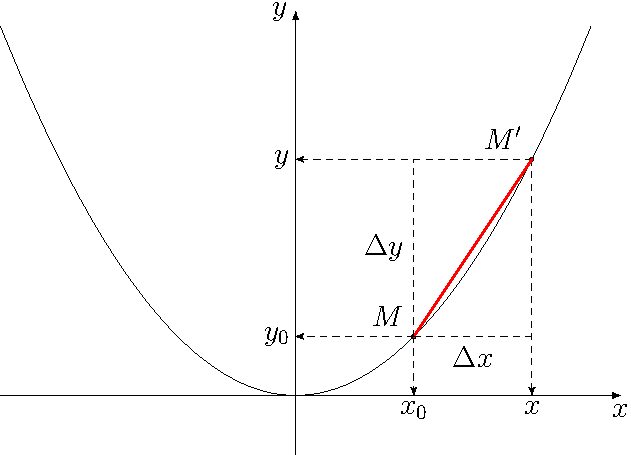
\includegraphics[page=1,scale=0.75]{analytic_geometry/int2.pdf}
	\caption{Hệ số góc (trường hợp 1)}
	\label{int2a}
\end{figure}

Tiếp theo, xét hình \ref{int2b}, ta thấy đường thẳng $MM'$ ngày càng tiến sát lại với đường cong. Như vậy, khi $\Delta x$ tiến tới 0 thì đường thẳng $MM'$ cắt đường cong tại hai điểm càng sát nhau. Đến khi hai điểm đó trùng nhau, đường thẳng $MM'$ chỉ đi qua đúng một điểm thuộc đường cong và khi đó $MM'$ trở thành tiếp tuyến của đường cong tại điểm $M = (x_0, y_0)$.

\begin{figure}[ht]
	\centering
	\includegraphics[page=2,scale=0.75]{analytic_geometry/int2.pdf}
	\caption{Hệ số góc (trường hợp 2)}
	\label{int2b}
\end{figure}

Khi đó $f'(x_0)$ là tangent của góc hợp bởi $MM'$ và trục hoành $Ox$, hay nói cách khác là \textit{hệ số góc} của đường tiếp tuyến. Thêm nữa $f'(x_0) = \dfrac{\Delta y}{\Delta x} = \dfrac{y - y_0}{x - x_0}$ nên phương trình đường tiếp tuyến đi qua $M = (x_0, y_0)$ là
\begin{equation}
	y = f'(x_0) (x - x_0) + y_0
\end{equation}

\section{Tích phân}

Tích phân là khái niệm quan trọng trong giải tích. Sau đây sẽ trình bày cách tính tích phân theo tổng Riemann.

\subsection*{Tích phân và phân chia diện tích}

Xét phương trình của một đường cong $y = f(x) > 0$ trên đoạn $[a, b]$.

Theo định nghĩa, tích phân từ $a$ tới $b$ là diện tích phần hình phẳng giới hạn bởi đường cong $y = f(x)$, trục hoành $Ox$ và hai trục đứng $x = a$, $x = b$.

Ờ hình \ref{int1}, diện tích phần tô màu xám là tích phân từ -2 tới 2 của hàm số $f(x) = -x^2 + 4$.

\begin{figure}[ht]
	\centering
	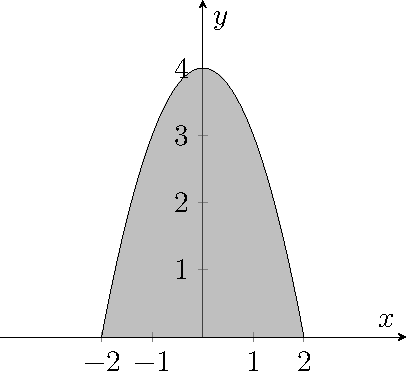
\includegraphics[page=1]{analytic_geometry/int1.pdf}
	\caption{Tích phân từ -2 tới 2 của $f(x) = -x^2 + 4$}
	\label{int1}
\end{figure}

Chúng ta có thể tính diện tích hình chữ nhật, hình thang, hình vuông. Vậy có cách nào để tính diện tích một hình giới hạn bởi các đường cong bất kì không? Có đấy. Chúng ta sẽ tính xấp xỉ bằng tổng diện tích các hình chữ nhật.

Ví dụ với hàm số $f(x) = -x^2 + 4$ ở trên, ta chia đoạn $[a, b]$ thành $n$ phần bằng nhau \[a = x_0 < x_1 < \ldots < x_{n-1} < x_n = b\]
Trong đó $x_{i+1} - x_i$ cố định và bằng $\dfrac{b-a}{n}$.

Đối với hình \ref{int2} ta xấp xỉ bằng 7 hình chữ nhật. Đối với hình \ref{int3} ta xấp xỉ bằng 15 hình chữ nhật. Đối với hình \ref{int4} ta xấp xỉ bằng 31 hình chữ nhật. 

\begin{figure}[htb]
	\centering
	\includegraphics[page=2]{analytic_geometry/int1.pdf}
	\caption{Xấp xỉ diện tích bởi 7 hình chữ nhật}
	\label{int2}
\end{figure}

\begin{figure}[htb]
	\centering
	\includegraphics[page=3]{analytic_geometry/int1.pdf}
	\caption{Xấp xỉ diện tích bởi 15 hình chữ nhật}
	\label{int3}
\end{figure}

\begin{figure}[htb]
	\centering
	\includegraphics[page=4]{analytic_geometry/int1.pdf}
	\caption{Xấp xỉ diện tích bởi 31 hình chữ nhật}
	\label{int4}
\end{figure}

Càng dùng nhiều hình chữ nhật, tổng diện tích của chúng càng gần với diện tích cần tìm, hay là tích phân cần tìm.

Ở ba hình trên, mỗi hình chữ nhật trong đó có chiều rộng bằng nhau là $\dfrac{b-a}{n}$ với $n$ là số đoạn. Chiều dài là $f(x_i)$ với $x_i = a + \dfrac{b-a}{n} i$, $i = 1, 2, \ldots, n$ (biên sau).

Cụ thể hơn, hình chữ nhật từ $x_{i-1}$ tới $x_i$ sẽ có chiều dài là $f(x_i)$ và chiều rộng là $\dfrac{b-a}{n}$. % Việc chọn chiều dài không bắt buộc phải chọn biên sau. Chúng ta hoàn toàn có thể chọn chiều dài là $f(x_{i-1})$, hoặc $\max f(x)$, $\min f(x)$ trên đoạn $[x_{i-1}, x_i]$.

Khi đó, tổng diện tích của các hình chữ nhật là
\begin{equation}
	\sum_{i=1}^n (x_{i} - x_{i-1}) f(x_i) = \sum_{i=1}^n \frac{b-a}{n} f(x_i)
\end{equation}

Khi số lượng hình chữ nhật tăng lên tới vô hạn thì tổng diện tích sẽ tiến tới diện tích chính xác của hình cần tìm, hay nói cách khác là tích phân. Do đó kết quả sẽ là
\begin{equation}
	\int\displaylimits_{a}^{b} f(x)\,dx = \lim_{n \to \infty} \sum_{i=1}^{n} \frac{b-a}{n} f(x_i), \quad x_i = a + \frac{b-a}{n} i
\end{equation}

\subsection*{Ví dụ tính tích phân qua tổng Riemann}

Ví dụ, tính tích phân từ -2 tới 2 của hàm số $f(x) = -x^2 + 4$ ở trên. Ta có $b = 2$ và $a = -2$ nên \begin{align*}
	\frac{b-a}{n} f(x_i) = & \frac{4}{n} \Bigl(-\Bigl(-2+\frac{4}{n} i\Bigr)^2 + 4\Bigr) \\ = & \frac{4}{n}\Bigl( -4 + \frac{16}{n} i - \frac{16}{n^2} i^2 + 4\Bigr) \\ = & \frac{64}{n} \Bigl( \frac{i}{n} - \frac{i^2}{n^2} \Bigr)
\end{align*}

Tính tổng $i$ từ 1 tới $n$ ta có $\displaystyle{\sum_{i=1}^{n} i = \frac{n(n+1)}{2}}$.

Tính tổng $i^2$ từ 1 tới $n$ ta có $\displaystyle{\sum_{i=1}^{n} i^2 = \frac{n(n+1)(2n+1)}{6}}$.

Suy ra
\begin{align*}
	\sum_{i=1}^n \frac{64}{n} \Bigl(\frac{i}{n} - \frac{i^2}{n^2}\Bigr) = & \frac{64}{n^2} \sum_{i=1}^n i - \frac{64}{n^3} \sum_{i=1}^{n} i^2 \\ & = -\frac{64}{n^2} \cdot \frac{n(n+1)}{2} - \frac{64}{n^3} \cdot \frac{n(n+1)(2n+1)}{6}
\end{align*}

Khi $n$ tiến tới vô cực thì biểu thức trên tiến tới $\dfrac{64}{2} - \dfrac{64 \cdot 2}{6} = \dfrac{32}{3}$. Đây chính là giá trị của tích phân $\displaystyle{\int\displaylimits_{-2}^2 (-x^2 + 4) \, dx}$.